\chapter{Single-node Computation}

\section{Introduction}

In this chapter we describe all base objects (matrices, vectors and stencils) for computation on single-node (shared-memory) systems. A typical configuration is presented on Figure \ref{single-node}.

\begin{figure}[!ht]
\centering
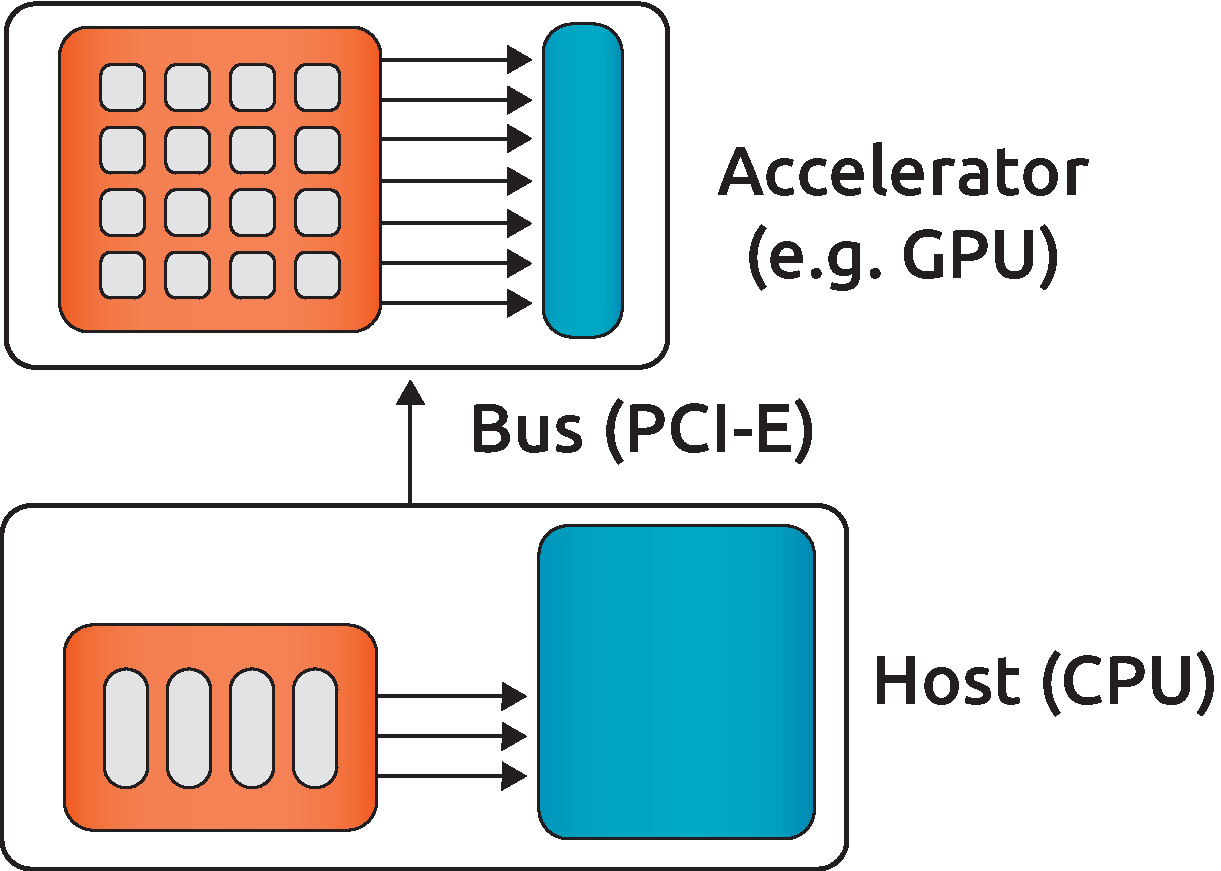
\includegraphics[width=0.6\textwidth]{./fig/single-node.pdf}
\caption{A typical single-node configuration, where gray-boxes represent the cores, blue-boxes represent the memory, arrows represent the bandwidth}
\label{single-node}
\end{figure}

The compute node contains none, one or more accelerators. The compute node could be any kind of shared-memory (single, dual, quad CPU) system. Note that the memory of the accelerator and of the host can be physically different.

\section{Code Structure}

The \emph{Data} is an object, pointing to the \emph{BaseMatrix} class. The pointing is coming from either a \emph{HostMatrix} or an \emph{AcceleratorMatrix}. The \emph{AcceleratorMatrix} is created by an object with an implementation in each of the backends (CUDA, OpenCL, Xeon Phi) and a matrix format. Switching between host or accelerator matrix is performed in the \emph{LocalMatrix} class. The \emph{LocalVector} is organized in the same way.

\begin{figure}[!ht]
\centering
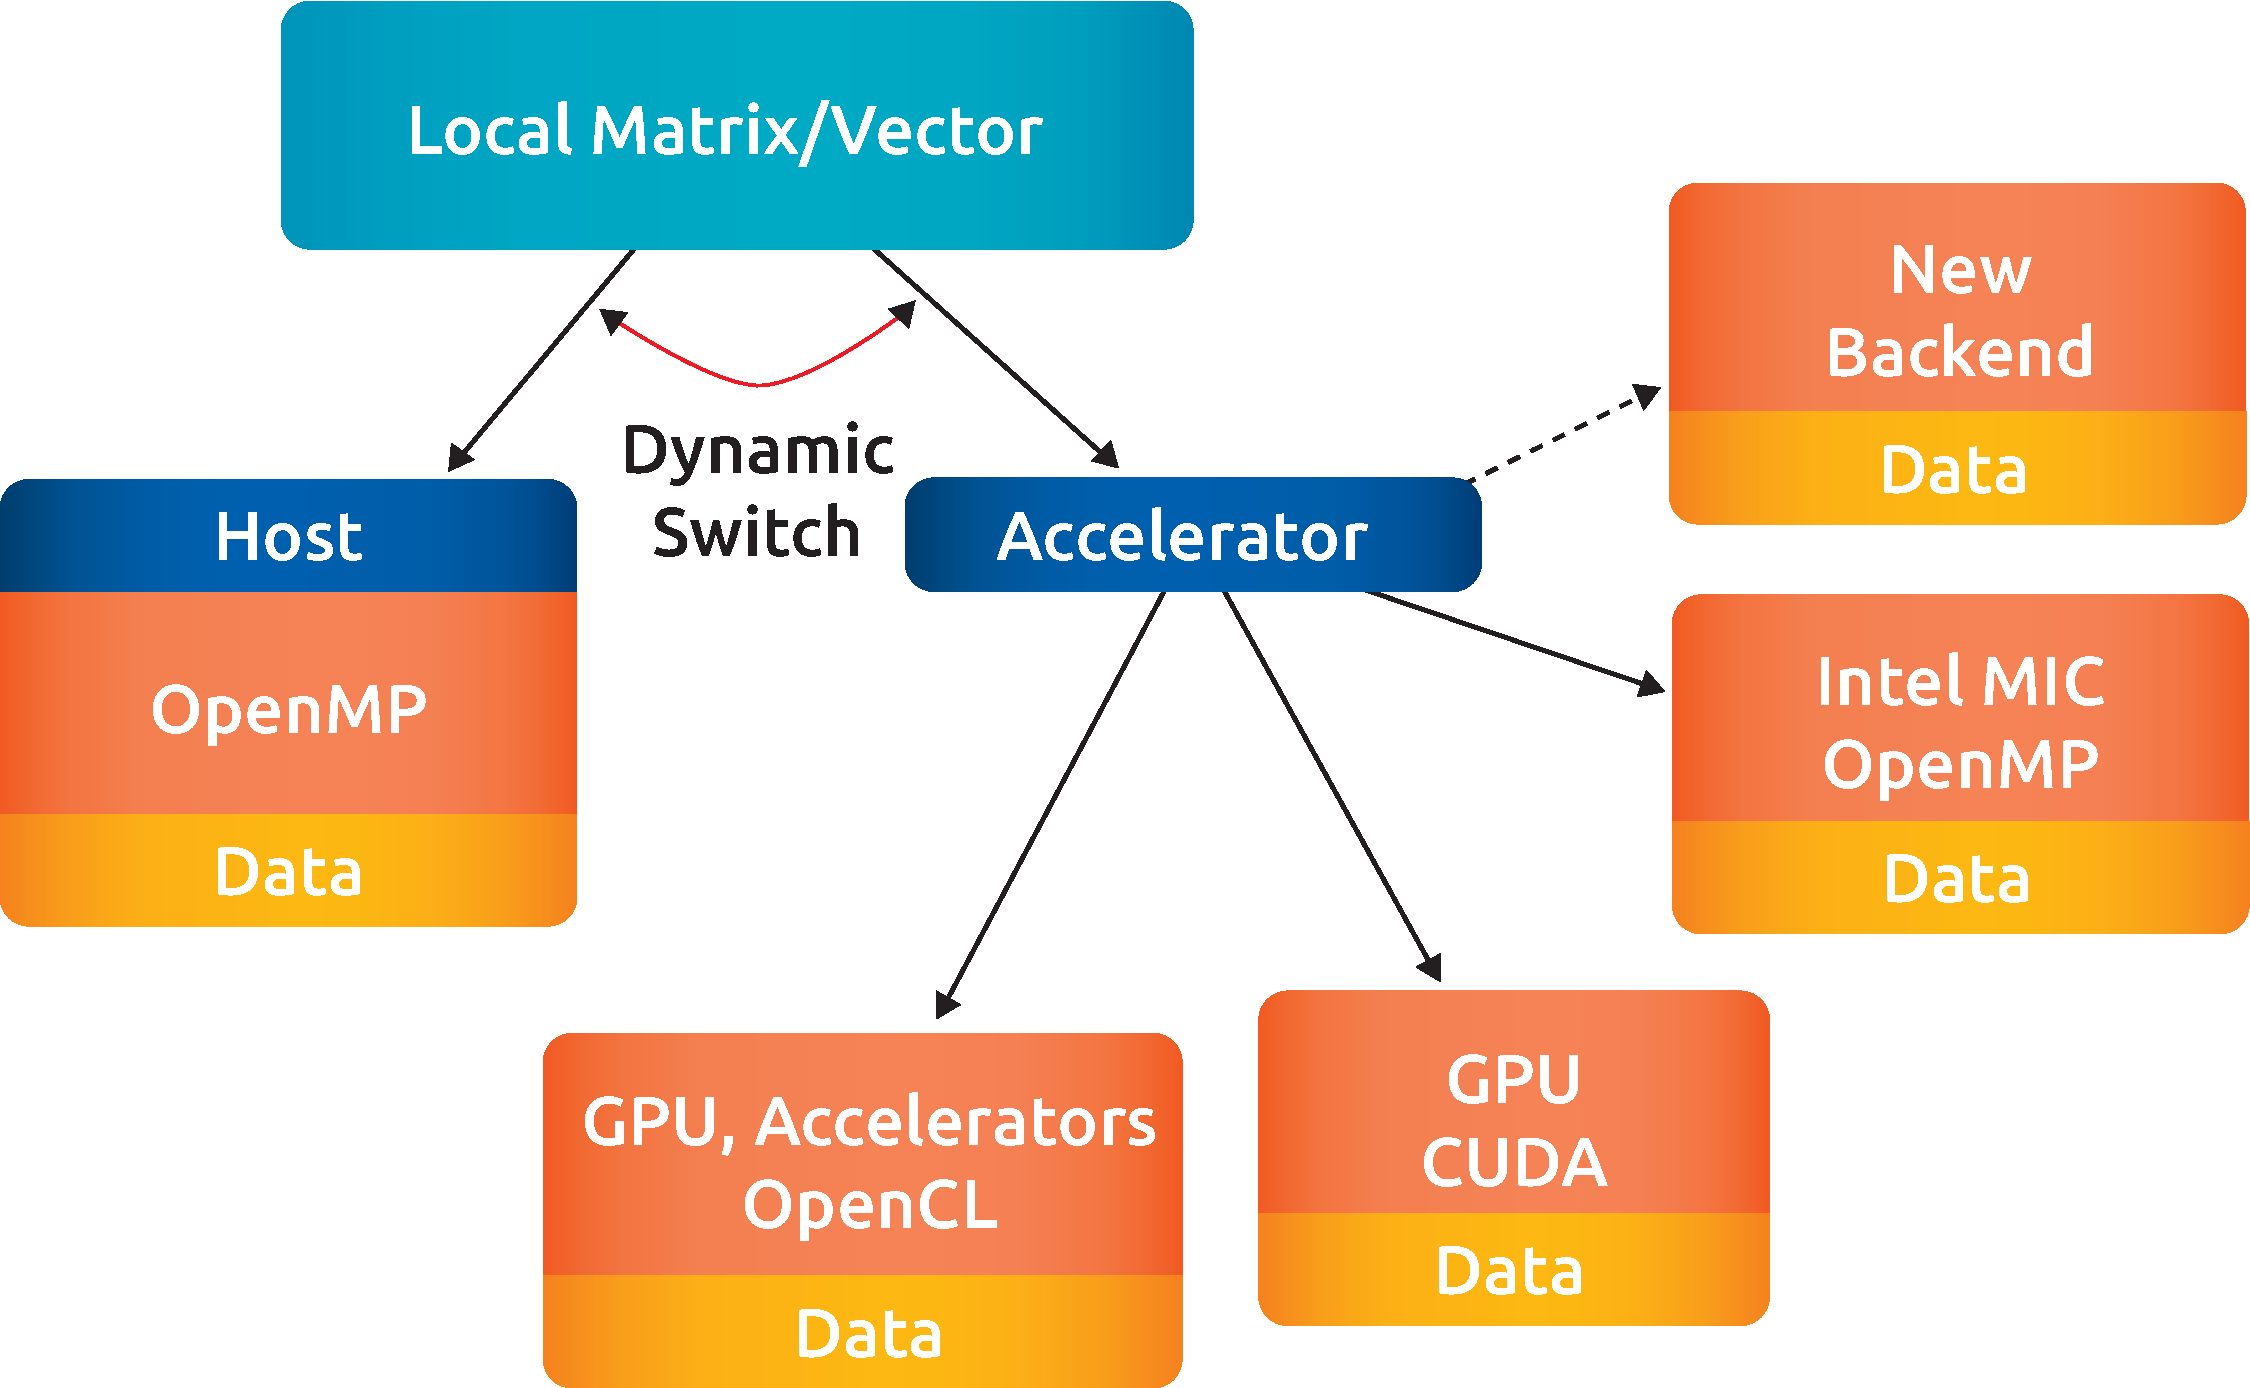
\includegraphics[width=0.6\textwidth]{./fig/local_obj.pdf}
\caption{Local Matrices and Vectors}
\label{paralution-local}
\end{figure}

\begin{figure}[!ht]
\centering
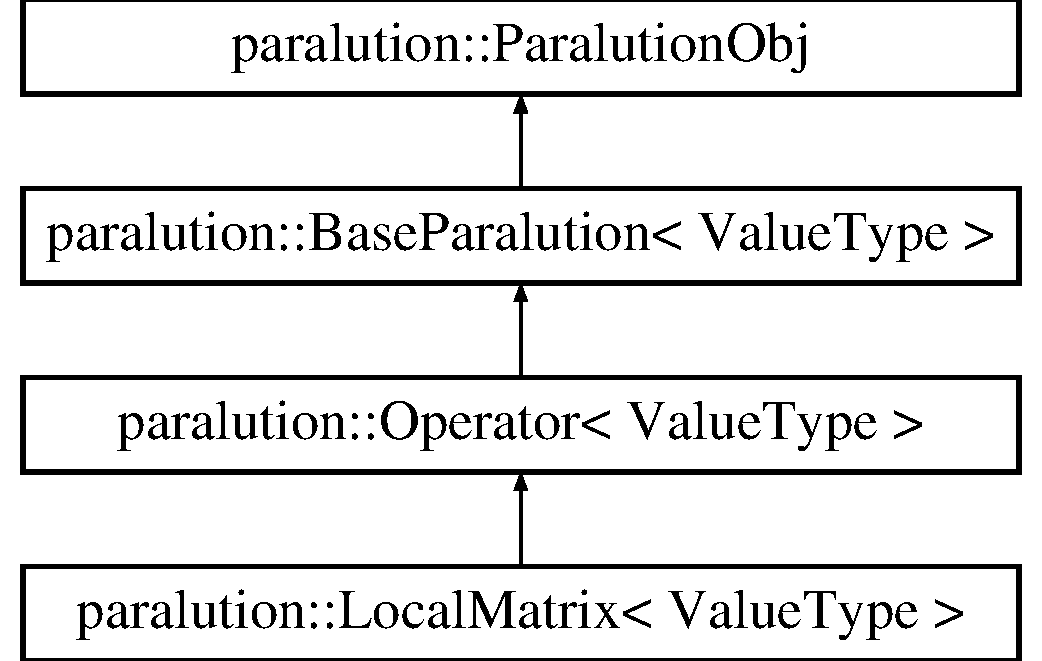
\includegraphics[width=0.33\textwidth]{./fig/body/classparalution_1_1_local_matrix.pdf}
\hspace{7mm}
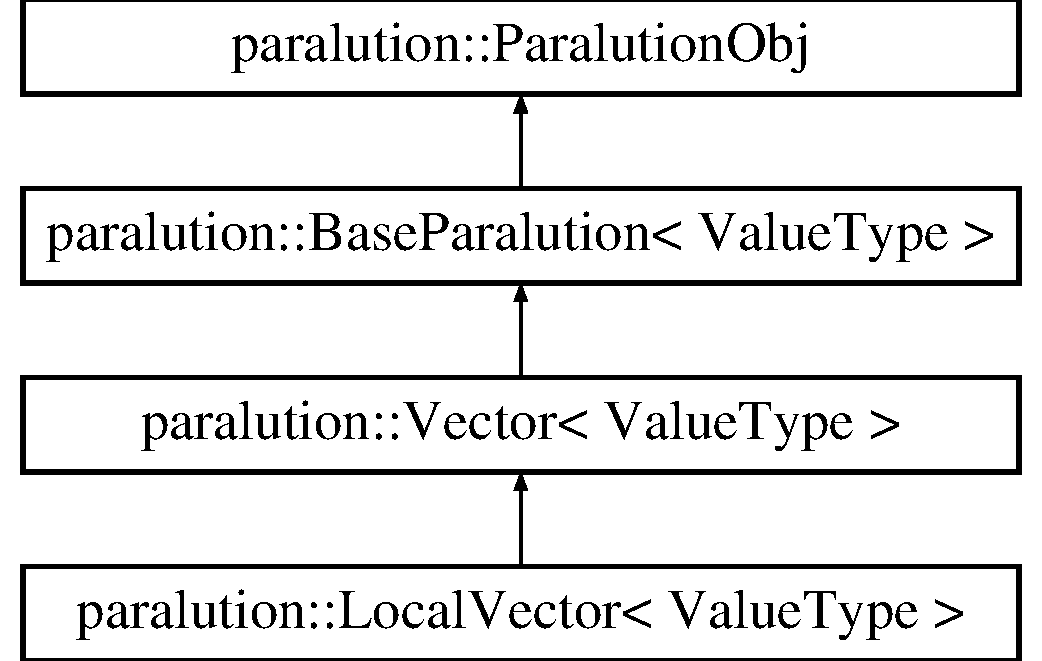
\includegraphics[width=0.33\textwidth]{./fig/body/classparalution_1_1_local_vector.pdf}
\caption{LocalMatrix and Local Vector}
\end{figure}

Each matrix format has its own class for the host and for each accelerator backend. All matrix classes are derived from the \emph{BaseMatrix} which provides the base interface for computation as well as for data accessing, see Figure\ref{BaseMatrix}. The GPU (CUDA backend) matrix structure is presented in Figure \ref{GPUMatrix}, all other backend follows the same organization.

\begin{figure}[!ht]
\centering
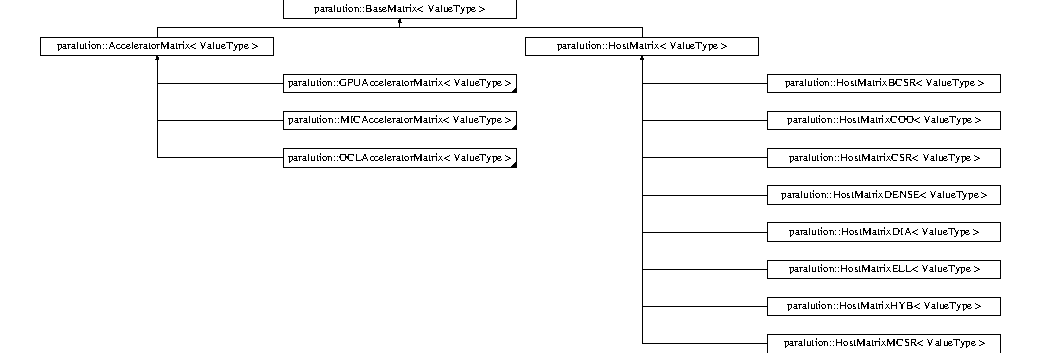
\includegraphics[width=1.0\textwidth]{./fig/body/classparalution_1_1_base_matrix.pdf}
\caption{BaseMatrix}
\label{BaseMatrix}
\end{figure}

\begin{figure}[!ht]
\centering
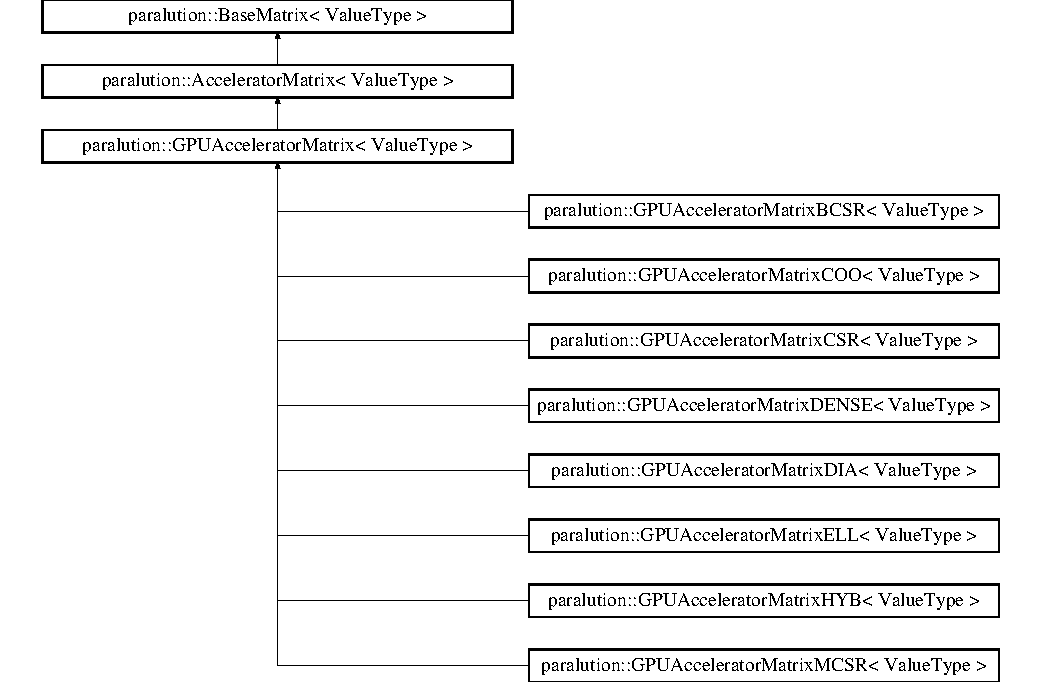
\includegraphics[width=0.7\textwidth]{./fig/body/classparalution_1_1_g_p_u_accelerator_matrix.pdf}
\caption{GPUAcceleratorMatrix (CUDA)}
\label{GPUMatrix}
\end{figure}


\section{Value Type}

The value (data) type of the vectors and the matrices is defined as a template. The matrix can be of type \emph{float} (32-bit), \emph{double} (64-bit) and \emph{complex} (64/128-bit). The vector can be \emph{float} (32-bit), \emph{double} (64-bit), \emph{complex} (64/128-bit) and \emph{int} (32/64-bit). The information about the precision of the data type is shown in the \emph{Print()} function.

\section{Complex Support}
\label{complex-support}

PARALUTION supports complex computation in all functions due to its internal template structure. The host implementation is based on the  \emph{std::complex}. In binary, the data is the same also for the CUDA and for the OpenCL backend.

\section{Allocation and Free}

The allocation functions require a name of the object (this is only for information purposes) and corresponding size description for vector and matrix objects.

\lstinputlisting[title="Vector allocation/free"]{./src/vector_allocation.cpp}

\lstinputlisting[title="Matrix allocation/free"]{./src/matrix_allocation.cpp}


\section{Matrix Formats}

Matrices where most of the elements are equal to zero are called sparse. In most practical applications the number of non-zero entries is proportional to the size of the matrix (e.g. typically, if the matrix $A$ is $\mathbb{R}^{N \times N}$ then the number of elements are of order $O(N)$). To save memory, we can avoid storing the zero entries by introducing a structure corresponding to the non-zero elements of the matrix. PARALUTION supports sparse CSR, MCSR, COO, ELL, DIA, HYB and dense matrices (DENSE). 

To illustrate the different format, let us consider the following matrix in Figure~\ref{sparse-matrix-example}.
%
%\[
%A=
%\begin{bmatrix}
%  1 & 2 & 0 &11 & 0\\
%  0 & 3 & 4 & 0 & 0\\
%  0 & 5 & 6 & 7 & 0\\
%  0 & 0 & 0 & 8 & 0\\
%  0 & 0 & 0 & 9 &10\\
%\end{bmatrix},
%\]
%
\begin{figure}[!ht]
\centering
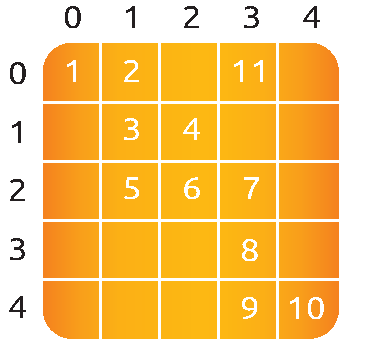
\includegraphics[width=0.3\textwidth]{./fig/mat/matrix.pdf}
\caption{A sparse matrix example}
\label{sparse-matrix-example}
\end{figure}
%

Here the matrix is $A$ $\in$ $\mathbb{R}^{5 \times 5}$ with $11$ non-zero entries. The indexing in all formats described below are zero based (i.e. the index values starts at $0$, not with $1$).

\textbf{\emph{Note}} The functionality of every matrix object is different and depends on the matrix format. The CSR format provides the highest support for various functions. For a few operations an internal conversion is performed, however, for many routines an error message is printed and the program is terminated.

\textbf{\emph{Note}} In the current version, some of the conversions are performed on the host (disregarding the actual object allocation - host or accelerator).

\lstinputlisting[title="Conversion between matrix formats"]{./src/matrix_convert.cpp}
\lstinputlisting[title="Conversion between matrix formats (alternative)"]{./src/matrix_convert2.cpp}

\subsection{Coordinate Format -- COO}

The most intuitive sparse format is the coordinate format (COO). It represent the non-zero elements of the matrix by their coordinates, we need to store two index arrays (one for row and one for column indexing) and the values. Thus, our example matrix will have the following structure:

\begin{figure}[!ht]
\centering
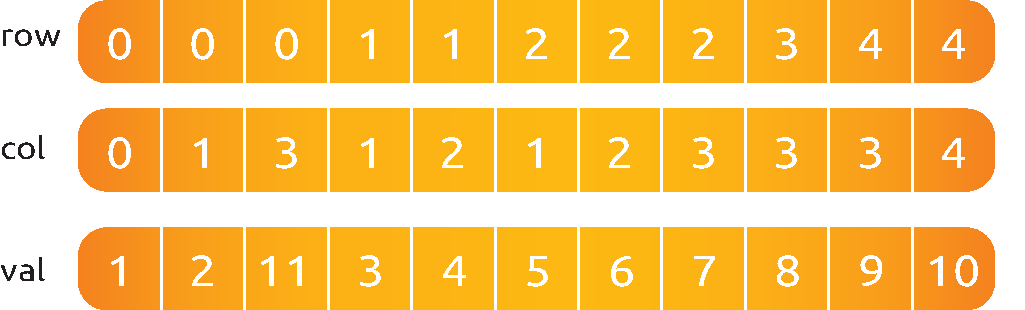
\includegraphics[width=0.5\textwidth]{./fig/mat/coo.pdf}
\caption{Sparse matrix in COO format}
\end{figure}

\subsection{Compressed Sparse Row/Column Format -- CSR/CSC}

One of the most popular formats in many scientific codes is the compressed sparse row (CSR) format. In this format, we do not store the whole row indices but we only save the offsets to positions. Thus, we can easily jump to any row and we can access sequentially all elements there. However, this format does not allow sequential accessing of the column entries.

\begin{figure}[!ht]
\centering
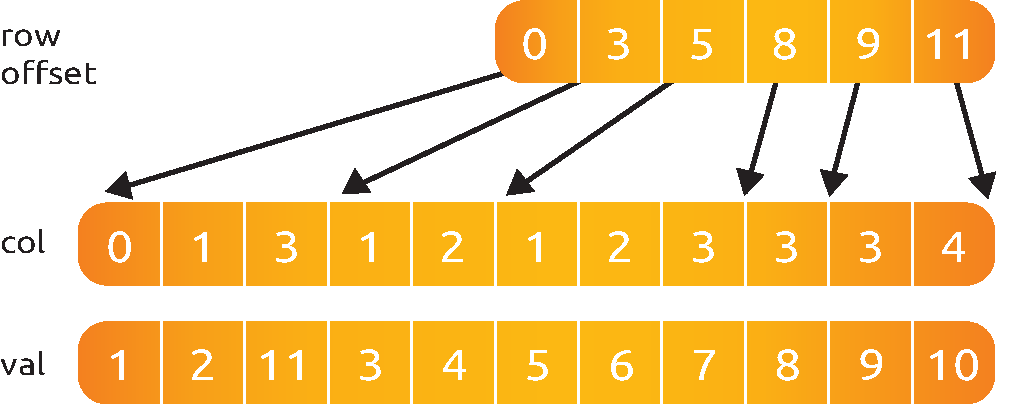
\includegraphics[width=0.5\textwidth]{./fig/mat/csr.pdf}
\caption{Sparse matrix in CSR format}
\end{figure}

Analogy to this format is the compressed sparse column (CSC), where we represent the offsets by the column -- it is clear that we can traverse column elements sequentially. 

In many finite element (difference/volumes) applications, the diagonal elements are non-zero. In such cases, we can store them at the beginning of the value arrays. This format is often referred as modified compressed sparse row/column (MCSR/MCSC).

\subsection{Diagonal Format -- DIA}

If all (or most) of the non-zero entries belong to a few diagonals of matrix, we can store them with the responding offsets. In our example, we have $4$ diagonal, the main diagonal (denoted with $0$ offset) is fully occupied while the others contain zero entries.

\begin{figure}[!ht]
\centering
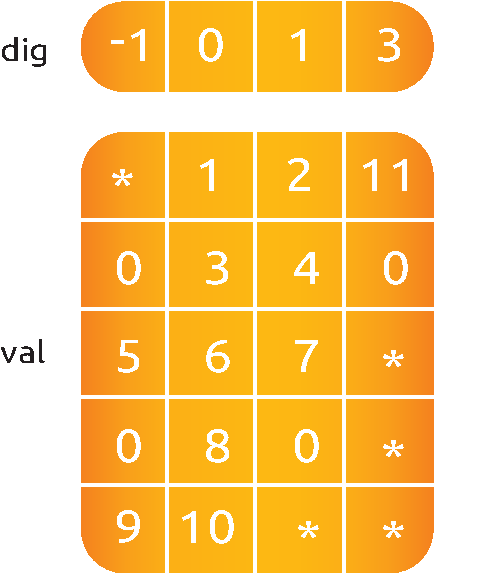
\includegraphics[width=0.3\textwidth]{./fig/mat/dia.pdf}
\caption{Sparse matrix in DIA format}
\end{figure}

Please note, that the values in this format are stored as array with size $D \times N_{D}$, where $D$ is the number of diagonals in the matrix and $N_{D}$ is the number of elements in the main diagonal. Since, not all values in this array are occupied - the not accessible entries are denoted with star, they correspond to the offsets in the diagonal array (negative values represent offsets from the beginning of the array).


\subsection{ELL Format}

The ELL format can be seen as modification of the CSR, where we do not store the row offsets. Instead, we have a fixed number of elements per row.

\begin{figure}[!ht]
\centering
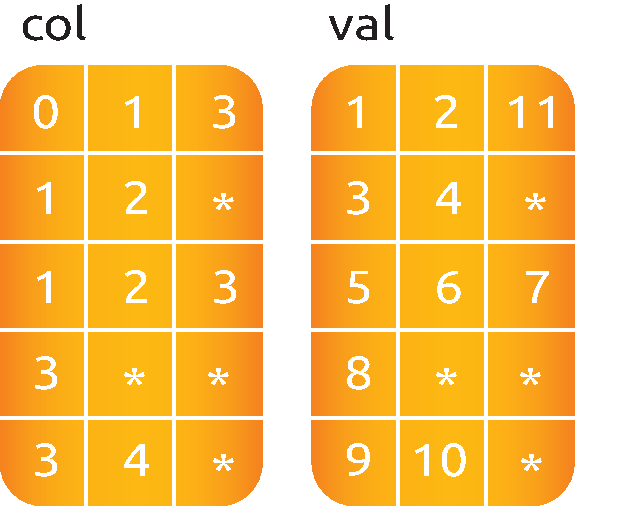
\includegraphics[width=0.35\textwidth]{./fig/mat/ell.pdf}
\caption{Sparse matrix in ELL format}
\end{figure}

\subsection{HYB Format}

As you can notice the DIA and ELL cannot represent efficiently completely unstructured sparse matrix. To keep the memory footprint low DIA requires the elements to belong to a few diagonals and the ELL format needs fixed number of elements per row. For many applications this is a too strong restriction. A solution to this issue is to represent the more regular part of the matrix in such a format and the remaining part in COO format.

The HYB format, implemented in PARALUTION, is a mix between ELL and COO, where the maximum elements per row for the ELL part is computed by nnz/num row. 

\subsection{Memory Usage}

The memory footprint of the different matrix formats is presented in the following table. Here, we consider a $N \times N$ matrix where the number of non-zero entries are denoted with $NNZ$.

\begin{table}[ht]
\centering
\begin{tabular}{l l l}
\hline\noalign{\smallskip}
Format & Structure & Values \\
\noalign{\smallskip}\hline\noalign{\smallskip}
Dense & --  & $N \times N$ \\
COO & $2 \times NNZ$  & $NNZ$ \\
CSR & $N+1 + NNZ$     & $NNZ$ \\
ELL & $M \times N$    & $M \times N$ \\
DIA & $D$             & $D \times N_{D}$ \\
\noalign{\smallskip}\hline\noalign{\smallskip}
\end{tabular}
\end{table}

For the ELL matrix $M$ characterizes the maximal number of non-zero elements per row and for the DIA matrix $D$ defines the number of diagonals and $N_D$ defines the size of the main diagonal.


\subsection{Backend support}

\begin{table}[H]
\begin{tabular}{l|l|l|l|l}
\multicolumn{1}{c|}{} & \multicolumn{1}{c|}{\begin{tabular}[c]{@{}c@{}}Host\end{tabular}} & \multicolumn{1}{c|}{\begin{tabular}[c]{@{}c@{}}CUDA\end{tabular}} & \multicolumn{1}{c|}{\begin{tabular}[c]{@{}c@{}}OpenCL\end{tabular}} & \multicolumn{1}{c}{\begin{tabular}[c]{@{}c@{}}MIC/Xeon Phi\end{tabular}} \\ \hline
% Format           |  Host  |  CUDA  |  OpenCL  |  Xeon Phi
CSR                & Yes    & Yes    & Yes      & \multicolumn{1}{l|}{Yes}\\ \hline
COO                & Yes    & Yes    & Yes      & \multicolumn{1}{l|}{Yes}\\ \hline
ELL                & Yes    & Yes    & Yes      & \multicolumn{1}{l|}{Yes}\\ \hline
DIA                & Yes    & Yes    & Yes      & \multicolumn{1}{l|}{Yes}\\ \hline
HYB                & Yes    & Yes    & Yes      & \multicolumn{1}{l|}{Yes}\\ \hline
DENSE              & Yes    & Yes    & Yes      & \multicolumn{1}{l|}{No}\\ \hline
BCSR               & No     & No     & No       & \multicolumn{1}{l|}{No}\\ \hline
\end{tabular}
\end{table}

\section{I/O}

The user can read and write matrix files stored in Matrix Market Format \cite{mm}.
\lstinputlisting[title="I/O MTX Matrix"]{./src/matrix_io.cpp}

Matrix files in binary format are also supported for the compressed sparse row storage format.
\lstinputlisting[title="I/O CSR Binary Matrix"]{./src/matrix_io_binary.cpp}
The binary format stores the CSR relevant data as follows
\lstinputlisting[title="CSR Binary Format"]{./src/io_binary.cpp}

The vector can be read or written via ASCII formatted files
\lstinputlisting[title="I/O ASCII Vector"]{./src/vector_io.cpp}

\section{Access}

\begin{table}[H]
\begin{tabular}{l|l|l}
\multicolumn{1}{c|}{ValueType} & Computation & Available \\ \hline
D,F,I,C                        & H           & S,M    
\end{tabular}
\end{table}


The elements in the vector can be accessed via \emph{[]} operators when the vector is allocated on the host. In the following example, a vector is allocated with 100 elements and initialized with $1$ for all odd elements and $-1$ for all even elements.
\lstinputlisting[title="Vector element access"]{./src/vector_access.cpp}

\textbf{\emph{Note}} Accessing elements via the \emph{[]} operators is slow. Use this for debugging only.

There is no direct access to the elements of matrices due to the sparsity structure. Matrices can be imported by a copy function, for CSR matrix this is \emph{CopyFromCSR()} and \emph{CopyToCSR()}.
\lstinputlisting[title="Matrix access"]{./src/matrix_access.cpp}

\section{Raw Access to the Data}

\begin{table}[H]
\begin{tabular}{l|l|l}
\multicolumn{1}{c|}{ValueType} & Computation & Available \\ \hline
D,F,I,C                        & H,C          & S,M    
\end{tabular}
\end{table}


For vector and matrix objects, you can have direct access to the raw data via pointers. You can set already allocated data with the \emph{SetDataPtr()} function. 

\lstinputlisting[title="Set allocated data to a vector"]{./src/vector_raw2.cpp}
\lstinputlisting[title="Set allocated data to a CSR matrix"]{./src/matrix_raw2.cpp}

With \emph{LeaveDataPtr()} you can obtain the raw data from the object. This will leave the object empty.

\lstinputlisting[title="Get (steal) the data from a vector"]{./src/vector_raw.cpp}
\lstinputlisting[title="Get (steal) the data from a CSR matrix"]{./src/matrix_raw.cpp}

After calling the \emph{SetDataPtr*()} functions (for Vectors or Matrices), the passed pointers will be set to NULL.

\textbf{\emph{Note}} If the object is allocated on the host then the pointers from the \emph{SetDataPtr()} and \emph{LeaveDataPtr()} will be on the host, if the vector object is on the accelerator then the data pointers will be on the accelerator.

\textbf{\emph{Note}} If the object is moved to and from the accelerator then the original pointer will be invalid.

\textbf{\emph{Note}} Never rely on old pointers, hidden object movement to and from the accelerator will make them invalid.

\textbf{\emph{Note}} Whenever you pass or obtain pointers to/from a PARALUTION object, you need to use the same memory allocation/free functions, please check the source code for that (for Host \emph{src/utils/allocate\_free.cpp} and for Host/CUDA \emph{src/base/gpu/gpu\_allocate\_free.cu})

\section{Copy CSR Matrix Host Data}

\begin{table}[H]
\begin{tabular}{l|l|l}
\multicolumn{1}{c|}{ValueType} & Computation & Available \\ \hline
D,F,C                          & H,C,O       & S,M
\end{tabular}
\end{table}

If the CSR matrix data pointers are only accessible as constant, the user can create a PARALUTION matrix object and pass const CSR host pointers by using the \emph{CopyFromHostCSR()} function. PARALUTION will then allocate and copy the CSR matrix on the corresponding backend, where the original object was located at.


\section{Copy Data}

\begin{table}[H]
\begin{tabular}{l|l|l}
\multicolumn{1}{c|}{ValueType} & Computation & Available \\ \hline
D,F,I,C                        & H,C          & S,M    
\end{tabular}
\end{table}

The user can copy data to and from a local vector via the \emph{CopyFromData()} and \emph{CopyToData()} functions. The vector must be allocated before with the corresponding size of the data. 


\section{Object Info}

Information about the object can be printed with the \emph{Info()} function
\lstinputlisting[title="Vector/Matrix information"]{./src/info.cpp}
\lstinputlisting[title="Vector/Matrix information"]{./src/info.txt}
In this example, the matrix has been loaded, stored in CSR format, double precision, the library is compiled with CUDA support and no MKL, and the matrix is located on the host. The vector information is coming from another compilation of the library with no OpenCL/CUDA/MKL support.

\section{Copy}

\begin{table}[H]
\begin{tabular}{l|l|l}
\multicolumn{1}{c|}{ValueType} & Computation & Available \\ \hline
D,F,I,C                        & H,C,O,X     & S,M    
\end{tabular}
\end{table}


All matrix and vector objects provide a \emph{CopyFrom()} and a \emph{CopyTo()} function. The destination object should have the same size or be empty. In the latter case the object is allocated at the source platform.

\textbf{\emph{Note}} This function allows cross platform copying - one of the objects could be allocated on the accelerator backend.

\lstinputlisting[title="Vector copy"]{./src/copy.cpp}

\textbf{\emph{Note}} For vectors, the user can specify source and destination offsets and thus copy only a part of the whole vector into another vector.

\textbf{\emph{Note}} When copying a matrix - the source and destination matrices should be in the same format.
 
\section{Clone}

\begin{table}[H]
\begin{tabular}{l|l|l}
\multicolumn{1}{c|}{ValueType} & Computation & Available \\ \hline
D,F,I,C                        & H,C,O,X     & S,M    
\end{tabular}
\end{table}

The copy operators allow you to copy the values of the object to another object, without changing the backend specification of the object. In many algorithms you might need auxiliary vectors or matrices. These objects can be cloned with the function \emph{CloneFrom()}.

\lstinputlisting[title="Clone"]{./src/clone.cpp}

If the data of the object needs to be kept, then you can use the \emph{CloneBackend()} function to copy (clone) only the backend.

\lstinputlisting[title="Clone backend"]{./src/clone2.cpp}

\section{Check}

\begin{table}[H]
\begin{tabular}{l|l|l}
\multicolumn{1}{c|}{ValueType} & Computation & Available \\ \hline
D,F,I,C                        & H (CSR-only)& S,M    
\end{tabular}
\end{table}

Checks, if the object contains valid data via the \emph{Check()} function. For vectors, the function checks if the values are not infinity and not NaN (not a number). For the matrices, this function checks the values and if the structure of the matrix is correct.


\section{Sort}

\begin{table}[H]
\begin{tabular}{l|l|l}
\multicolumn{1}{c|}{ValueType} & Computation & Available \\ \hline
D,F,I,C                        & H (CSR-only)& S,M    
\end{tabular}
\end{table}

Sorts the column values in a CSR matrix via the \emph{Sort()} function.


\section{Keying}

\begin{table}[H]
\begin{tabular}{l|l|l}
\multicolumn{1}{c|}{ValueType} & Computation & Available \\ \hline
D,F,I,C                        & H (CSR-only)& S,M
\end{tabular}
\end{table}

Typically it is hard to compare if two matrices have the same (structure and values) or they just have the same structure. To do this, we provide a key function which generates three keys, for the row index, column index and for the values. An example is presented in the following Listing.

\lstinputlisting[title="Generating a matrix key"]{./src/key.cpp}



\section{Graph Analyzers}

\begin{table}[H]
\begin{tabular}{l|l|l}
\multicolumn{1}{c|}{ValueType} & Computation & Available \\ \hline
D,F,I,C                        & H (CSR-only)& S,M    
\end{tabular}
\end{table}


The following functions are available for analyzing the connectivity in graph of the underlying sparse matrix.

\begin{itemize}
\itemsep0em
\item (R)CMK reordering
\item Maximal independent set
\item Multi-coloring
\item ZeroBlockPermutation
\item Connectivity ordering
\end{itemize}

All graph analyzing functions return a permutation vector (int type) which is supposed to be used with the \emph{Permute()} and \emph{PermuteBackward()} functions in the matrix and vector classes.

The CMK (Cuthill--McKee) and RCMK (Reverse Cuthill--McKee) orderings minimize the bandwidth of a given sparse matrix.
\lstinputlisting[title="CMK ordering"]{./src/cmk.cpp}

The Maximal independent set (MIS) algorithm finds a set with maximal size which contains elements that do not depend on other elements in this set.
\lstinputlisting[title="MIS ordering"]{./src/mis.cpp}

The Multi-coloring (MC) algorithm builds a permutation (coloring the matrix) in such way that no two adjacent nodes in the sparse matrix are having the same color.
\lstinputlisting[title="MC ordering"]{./src/mc.cpp}

For saddle-point problems (i.e. matrices with zero-diagonal entries) the ZeroBlockPermutation maps all zero-diagonal elements to the last block of the matrix.
\lstinputlisting[title="Zero-Block-Permutation"]{./src/zbp.cpp}

Connectivity ordering returns a permutation which sorts the matrix by non-zero entries per row.
\lstinputlisting[title="Connectivity ordering"]{./src/conn.cpp}

Visualization of the graph analyzers can be found in Chapter~\ref{graph-analyzers}.

\section{Basic Linear Algebra Operations}

There are more functions and routines which matrix and vector objects can perform - for further specifications and API, check the doxygen documentation.

\vspace{6mm}
Matrix objects can also perform 
\begin{itemize}
\itemsep0em
\item Matrix-vector multiplication $x:=Ay$ -- \emph{Apply()} 
\item Matrix-vector multiplication and addition $x:=x+Ay$ -- \emph{ApplyAdd()}
\item Symmetric permutation -- \emph{Permute()}; \emph{PermuteBackward()}
\item Sub-matrix / diagonal / L / U extractions -- \emph{ExtractSubMatrix()}; \emph{ExtractSubMatrices()}; \emph{ExtractDiagonal()}; \emph{ExtractInverseDiagonal()}; \emph{ExtractU()}; \emph{ExtractL()}; \emph{ExtractColumnVector()} ; \emph{ExtractRowVector()}
\item Sparse triangular solvers (L,U,LL,LU) -- ; \emph{LSolve()}; \emph{LLSolve()}; \emph{LUSolve()}
\item Factorizations - 
\begin{itemize}
 \item ILU(0) -- ILU with no fill-ins -- \emph{ILU0()}
 \item ILU($p$) -- based on levels -- \emph{ILUpFactorize()};
 \item ILU($p$,$q$) -- based on power($q$)-pattern method -- via \emph{ILUpFactorize()}
 \item ILUT -- based on threshold \emph{ILUTFactorize()}
 \item IC0 -- Incomplete Cholesky with no fill-ins -- \emph{ICFactorize()}
\end{itemize}
\item FSAI computation -- \emph{FSAI()}
\item Symbolic power -- compute the pattern of $|A|^p$, where $|.|=a_{i,j}$ -- \emph{SymbolicPower()}
\item Sparse matrix-matrix addition (with the same or different sparsity patterns) -- \emph{MatrixAdd()}
\item Sparse matrix-matrix multiplication -- \emph{MatrixMult()}
\item Sparse matrix multiplication with a diagonal matrix (left and right multiplication) -- \emph{DiagonalMatrixMultL()}; \emph{DiagonalMatrixMultR()}
\item Compute the Gershgorin circles (eigenvalue approximations) -- \emph{Gershgorin()}
\item Compress (i.e. delete elements) under specified threshold, this function also updates the structure -- \emph{Compress()}
\item Transpose -- \emph{Transpose()}
\item Create a restriction matrix via restriction map -- \emph{CreateFromMap()}
\item Scale with scalar all values / diagonal / off-diagonal -- \emph{Scale()}; \emph{ScaleDiagonal()}; \emph{ScaleOffDiagonal()}
\item Add a scalar to all values / diagonal / off-diagonal -- \emph{AddScalar()}; \emph{AddScalarDiagonal()}; \emph{AddScalarOffDiagonal()}
\end{itemize}

\vspace{6mm}
Vector objects can also perform  
\begin{itemize}
\itemsep0em
\item Dot product (scalar product) -- \emph{Dot()}
\item Scaling -- \emph{Scale()}
\item Vector updates of types: $x:=x+\alpha y$, $x:=y+\alpha x$, $x:=\alpha x + \beta y$, $x:=\alpha x + \beta y + \gamma z$ -- \emph{ScaleAdd()}; \emph{AddScale()}; \emph{ScaleAddScale()}; \emph{ScaleAdd2()}
\item $L_1$, $L_2$ and $L_{\infty}$-norm -- \emph{Asum()}; \emph{Norm()}; \emph{Amax()} 
\item Sum -- \emph{Reduce()} 
\item Point-wise multiplication of two vector (element-wise multiplication) -- \emph{PointWiseMult()}
\item Permutations (forward and backward) -- \emph{Permute()}; \emph{PermuteBackward()}
\item Copy within specified permutation -- \emph{CopyFromPermute()}; \emph{CopyFromPermuteBackward()}
\item Restriction/prolongation via map -- \emph{Restriction()}; \emph{Prolongation()}
\item Initialized the vector with random values -- \emph{SetRandom()}
\item Power -- \emph{Power()}
\item Copy from double or float vector -- \emph{CopyFromDouble()}; \emph{CopyFromFloat()}
\end{itemize}


\section{Local Stencils}

Instead of representing the linear operator as a matrix, the user can use stencil operators. The stencil operator has to be defined manually in each class and backend. This is a necessary step in order to have good performance in terms of spatial-block technique and compiler optimization.

\begin{figure}[!ht]
\centering
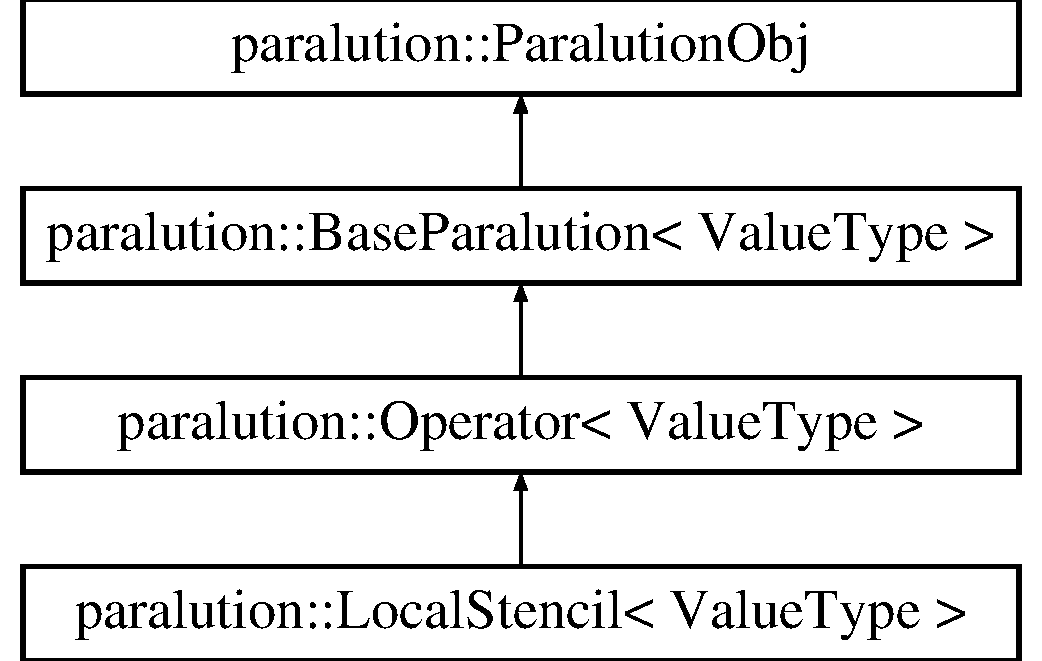
\includegraphics[width=0.33\textwidth]{./fig/body/classparalution_1_1_local_stencil.pdf}
\caption{Code structure of a host LocalStencil}
\end{figure}


\lstinputlisting[title="Example of 2D Laplace stencil"]{./src/stencil.cpp}
